\section{Experiments}\label{sec:experiments}

We investigated the impact of enforcing invariance on graph embeddings using three  datasets: Freebase15k-237\footnote{\tiny{\url{www.microsoft.com/en-us/download/details.aspx?id=52312}}}, MovieLens-1M\footnote{\tiny{\url{grouplens.org/datasets/movielens/1m/}}}, and an edge-prediction dataset derived from Reddit.\footnote{\tiny{\url{reddit.com}}} The specific dataset statistics are given in Table \ref{dataset_stats} and include the number of nodes, edges and types sensitive attributes considered for our experiments.


\subsection{Setup and datasets}

Before describing our experimental results, we first outline the key properties of the datasets we used, as well as specific encoders and edge-prediction loss functions used in the three different settings.  

In all experiments, we used multi-layer perceptrons (MLPs) with leaky ReLU activation functions \cite{xu2015empirical} as the discriminators, $D_k$. 
The Appendix contains details on the exact hyperparameters (e.g., number of layers and sizes) used for all the different experiments.
The Appendix also contains details on the training procedures (e.g., number of epochs).
Code to reproduce our results is included with the submission and will be made available upon publication. 

\subsubsection{Freebase-15k}

Freebase 15k-237 is a standard benchmark used for knowledge base completion \cite{toutanova2015representing}.
In this work, we use Freebase 15k-237 as a semi-synthetic testbed to evaluate the impact of adversarial regularization. 
Using the entity attribute labels from \citet{moon2017learning}, we used the $3$-most common attribute labels (e.g., /award/award\_nominee) as ``sensitive'' attributes.
The goal in this dataset is to perform the standard knowledge base completion task, while having the entity embeddings be invariant with respect to the ``sensitive'' attribute labels.
While synthetic, this dataset provides a useful reference point due to its popularity in the graph embedding literature. 

For our encoder and decoder, we follow \citet{ji2015knowledge}'s TransD approach, since we found this approach gave significant performance boosts compared to simpler models (e.g., TransE). 
In this model, the encoding of a node/entity depends on the edge relation being predicted, as well as on whether the entity is the head or tail in a relation (i.e., the edge direction matters).
In particular, the embedding of the head node (i.e., the source node) in an edge relation is given by:
\begin{equation}
    \enc(u, <u, r, v>) = (\mb{u}_p\mb{r}_p^\top + \mb{I}^{d \times d})\mb{u},
\end{equation}
where $\mb{u}, \mb{u}_p, \mb{r}_p \in \mathbb{R}^d$ are trainable embedding parameters and $\mb{I}^{d\times d}$ is a $d$-dimensional idenitity matrix. 
The encoding function for the tail node is defined analogously. 
The score function for this approach is given by
\begin{align*}\label{eq:transd}
s(<u, r, v>) = -\|\enc(u, <u, r, v>) + &\mb{r} \\ - \enc(v, <u, r,& v>)\|_2,
\end{align*}
where $\mb{r} \in \mathbb{R}^d$ is another trainable embedding parameter (one per relation). 
Finally, we use a standard max-margin loss with a single negative sample per positive edge:
\begin{equation}\label{eq:margin}
    L_{\textrm{edge}}(s(e), s(e^-)) = \max(0, 1 - s(e) + s(e)^-)
\end{equation}


\subsubsection{Movielens-1M}

Our second dataset is derived from the MovieLens-1M recommender system benchmark \CITE.
This is a standard recommender system benchmark, where the goal is to predict the rating that users assign movies.
However, unlike previous work, in our experiments we treat the user features (age\footnote{The ordinal age feature is mapped  to a categorical set by binning into 15 bins.}, gender, and occupation) as sensitive attributes (rather than as additional feature information for the recommendation task). 
Following \CITE\, we treat this recommendation task as an edge prediction problem between users and movies, viewing the different possible ratings as different edge relations. 

For this dataset we use a simple ``embedding-lookup'' encoder, where each user and movie is associated with a unique embedding vector in $\mathbb{R}^d$.
As a scoring function, we follow the recent state-of-the-art model of \CITE\ and use a  log-likelihood approach:
\begin{equation*}
    s(<u, r, m>) = \mb{z}_u^\top\mb{Q}_r\mb{z}_v-\log(\sum_{r' \in \mathcal{R}}\mb{z}_u^\top\mb{Q}_{r'}\mb{z}_v),
\end{equation*}
The relation matrices $\mb{Q}_r \in \mathbb{R}^{d \times d}$ are computed as:
\begin{equation*}
    \mb{Q}_r = a_{r, 1}\mb{P}_1 + a_{r,2}\mb{P}_2, 
\end{equation*}
where $a_{r, 1}, a_{r, 1} \in \R$ and $\mb{P}_1, \mb{P}_2 \in \R^{d \times d}$ are trainable parameters. 
In this case, the loss function involves no negative samples and is simple the negative of the log-likelihood score. 

\subsubsection{Reddit}

The final dataset we consider is based on the social media website Reddit \CITE---a popular, discussion-based website where users can post and comment on content in different topical communities, called ``subreddits''. 
For this dataset, we consider a traditional edge prediction task, where the goal is to predict interactions between users and subreddit communities. 

To construct the edge prediction task, we examined all comments from the month of November in $2017$, and we placed an edge between a user and a community if this user commented on that community at least once within this time period. 
We then took the $10$-core \CITE of this graph to remove low-degree nodes \CITE, which resulted in a graph with \red{X users, X communities, and X edges}.
Given this graph, the main task is to train an edge-prediction model on $90\%$ of the user-subreddit edges and then predict missing edges in a held-out test set of the remaining edges.  

Reddit is a pseudonymous website with no public user attributes.  
Thus, to define sensitive attributes, we treat certain subreddit nodes as {\em sensitive nodes}, and the sensitive attributes for users are whether or not they have an edge connecting to these sensitive nodes.
In other words, the fairness objective in this setting is to force the model to be invariant to whether or not a user commented on a particular community. 
We sampled {\red sampling details} to construct these sensitive subreddits.
Note that this setting represents the extreme case where we want the model to be invariant with respect to the existence of particular edges in the input graph. 

As with MovieLens-1M, we use a simple ``embedding-lookup'' encoder. 
In this case, there is only a single relation type---indicating whether a Reddit user has commented on a ``subreddit'' community.
Thus, we employ a simple dot-product based scoring function
\begin{equation*}
    s(<u, r, v>) = \mb{z}_u^\top\mb{z}_v,
\end{equation*}
and we use a max-margin loss as in Equation \eqref{eq:margin}. 

\subsection{Results}

The goal of our experiments was to answer three questions:
\begin{enumerate}[label={(\bf Q\arabic*)}, topsep=0pt, parsep=0pt, leftmargin=25pt]
    \item \textbf{The cost of invariance}. What is the tradeoff between enforcing invariance on the representations and accuracy on the main edge prediction task?
    \item \textbf{The impact of compositionality.} How does the performance of a compositional approach, which jointly enforces fairness over a set of sensitive attributes, compare to a more traditional model that only enforces fairness on a single attribute?
    \item \textbf{Invariance on unseen combinations.} In settings with many sensitive attributes, is our approach able to enforce invariance even on combinations of sensitive attributes that it never saw during training? 
\end{enumerate}
Throughout these experiments, we rely on two essential baseline approaches: First, we compare against a baseline approach that does not include any invariance constraints, i.e., an approach with $\lambda=0$ that is equivalent to a standard, graph embedding model. 
Second, we compare against a non-compositional adversarial approach where we separately train $K$ distinct encoders and $K$ distinct adversaries for each of the $K$ sensitive attributes in the data. 
This non-compositional adversary is essentially an extension of \CITE's approach to the graph embedding domain. 

\subsubsection{The cost of invariance}
In order to quantify the extent to which the learned embeddings are invariant to the sensitive attributes (e.g., after adversarial training), we fix the compositional encoder $\compenc$ and train a new MLP classifier to predict the sensitive attributes from the filtered embeddings. 
We also evaluate the performance of these filtered embeddings on the main, edge prediction task. 
In the best case, a newly trained classifier should have random accuracy when attempting to predict the sensitive attributes from the filtered embeddings, but these embeddings should still provide strong performance on the main edge prediction task. 

Overall, we found that on the more realistic MovieLens-1M and Reddit datasets, our approach was able to achieve a favorable tradeoff---with the sensitive attributes being nearly impossible to predict from the filtered embeddings and the accuracy on the main edge prediction task being close to a baseline approach that does not include the invariance constraints. 






\begin{figure}
    \centering
    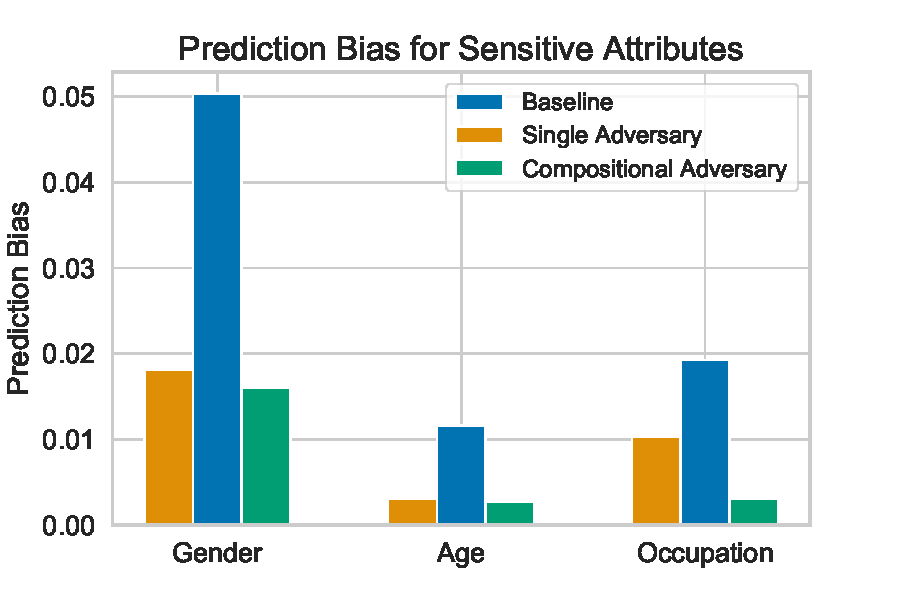
\includegraphics[width=1\linewidth]{icml2019_style/paper/plots/movielens1m_pred_bias.pdf}
    \caption{Prediction Bias for different Sensitive Attributes under three settings in MovieLens1M.}
    \label{fig:pred_bias}
\end{figure}

\begin{figure}
    \centering
    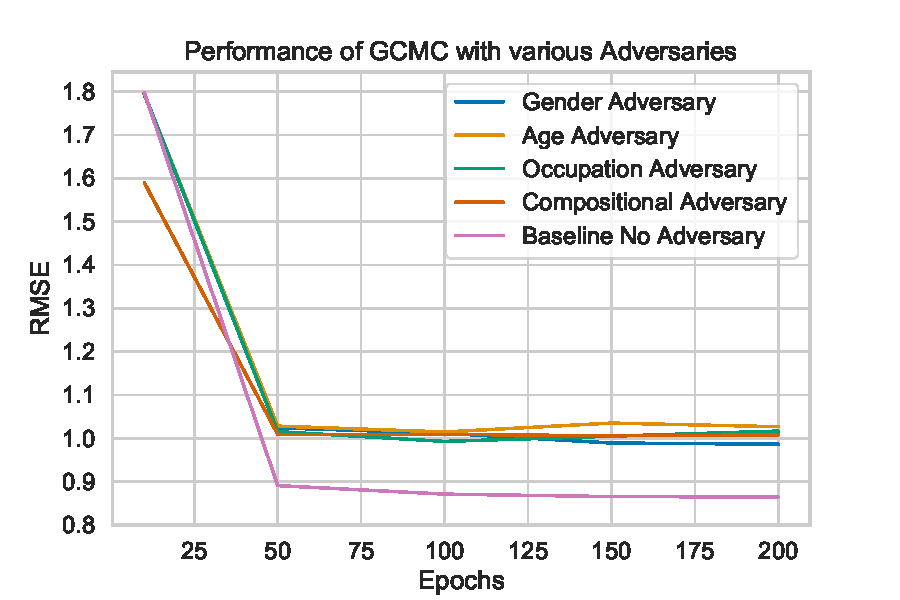
\includegraphics[width=1\linewidth]{icml2019_style/paper/plots/movielens1m_rmse.pdf}
    \caption{Performance of GCMC style encoder on MovieLens1M}
    \label{fig:rmse}
\end{figure}

\cut{
\begin{figure}
    \centering
    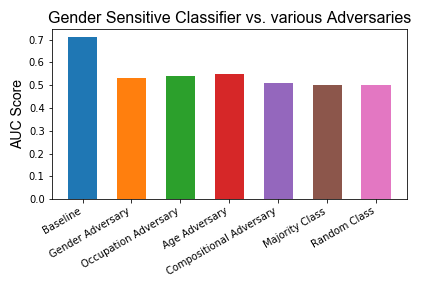
\includegraphics[width=1\linewidth]{icml2019_style/paper/plots/movielens1m_gender_auc.png}
    \caption{Gender Classifier AUC score versus various adversaries.}
    \label{fig:gender_f1}
\end{figure}

\begin{figure}
    \centering
    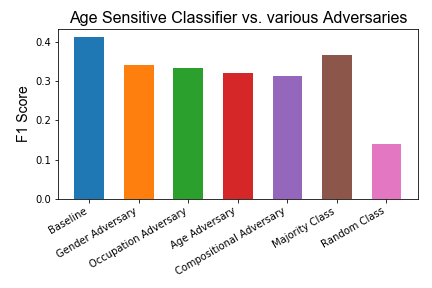
\includegraphics[width=1\linewidth]{icml2019_style/paper/plots/movielens1m_ageF1.png}
    \caption{Age Classifier F1 score versus various adversaries.}
    \label{fig:age_f1}
\end{figure}

\begin{figure}
    \centering
    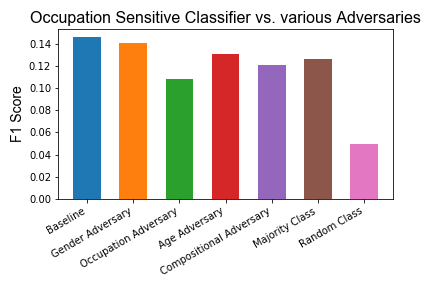
\includegraphics[width=1\linewidth]{icml2019_style/paper/plots/movielens1m_occF1.png}
    \caption{Occupation Classifier F1 score versus various adversaries.}
    \label{fig:occ_f1}
\end{figure}
}
\begin{figure}
    \centering
    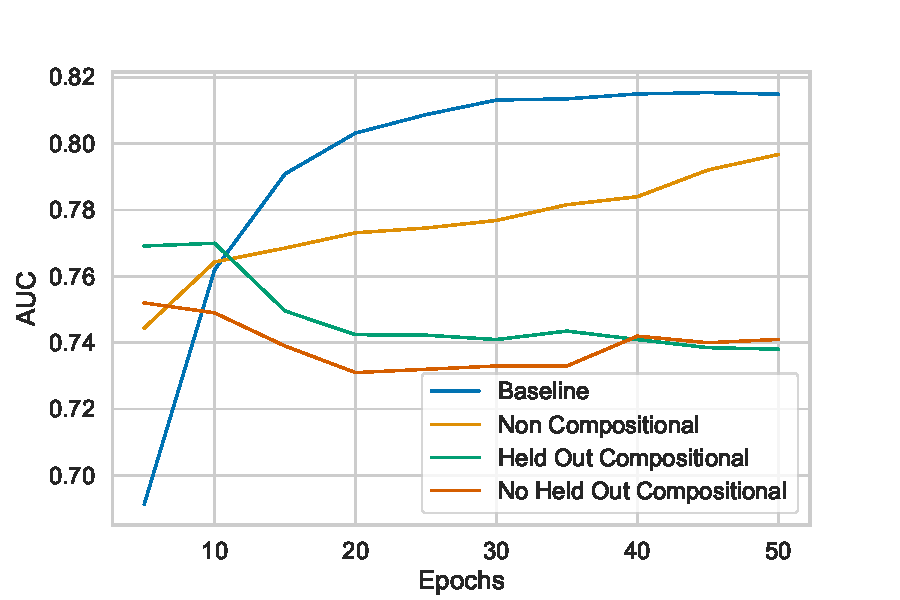
\includegraphics[width=1\linewidth]{icml2019_style/paper/plots/reddit_enc_auc.pdf}
    \caption{Reddit Encoder AUC score versus various Adversaries}
    \label{fig:reddit_enc_auc}
\end{figure}

\begin{figure}
    \centering
    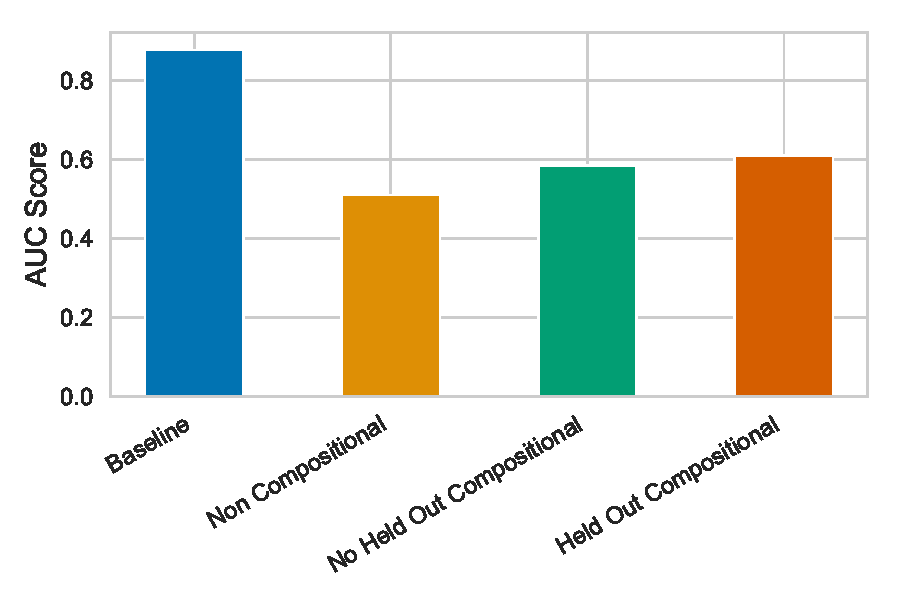
\includegraphics[width=1\linewidth]{icml2019_style/paper/plots/reddit_auc.pdf}
    \caption{Average Subreddit Classifier AUC score versus various Adversaries}
    \label{fig:reddit_auc}
\end{figure}

\begin{table*}[t]
\caption{Number of Head and Tail Nodes and Edges for each dataset. For FB15k-237 there is no distinction between Head and Tail nodes. We further indicate whether the sensitive attributes in each dataset are binary,multiclass or a combination of both.}
\label{sample-table}
\vskip 0.15in
\begin{center}
\begin{small}
\begin{sc}
\begin{tabular}{lcccccr}
\toprule
Dataset & \multicolumn{1}{p{1.5cm}}{\centering Head \\ Nodes} & \multicolumn{1}{p{1.5cm}}{\centering Tail \\ Nodes} & Edges & \multicolumn{1}{p{1.5cm}}{\centering Binary \\ Attributes?} & \multicolumn{1}{p{1.5cm}}{\centering Multiclass \\ Attributes?} \\
\midrule
FB15k-237    & 14,541& - & 237 &$\surd$ & $\times$ \\
MovieLens1M & 6,040&  3,900& 1,000,209&$\surd$ &$\surd$\\
Reddit Comments    & 366,797& 18938 &7,255,096 &$\surd$ & $\times$ \\
\bottomrule
\end{tabular}
\end{sc}
\end{small}
\end{center}
\vskip -0.1in
\label{dataset_stats}
\end{table*}



\begin{table*}[t]
\caption{Performance of Sensitive Attribute Classifiers versus various Adversaries. For Gender the score is AUC while for Age and Occupation the score is micro averaged F1. The columns represent the different adversaries while the rows are the respective classifiers.}
\label{sample-table}
\vskip 0.15in
\begin{center}
\begin{small}
\begin{sc}
\begin{tabular}{lccccccr}
\toprule
MovieLens1M & \multicolumn{1}{p{1.5cm}}{\centering Baseline \\ No Adversary} & \multicolumn{1}{p{1.5cm}}{\centering Gender \\ Adversary} & \multicolumn{1}{p{1.5cm}}{\centering Age \\ Adversary} & \multicolumn{1}{p{1.5cm}}{\centering Occupation \\ Adversary}&\multicolumn{1}{p{1.5cm}}{\centering Comp. \\ Adversary} & \multicolumn{1}{p{1.5cm}}{\centering Majority \\ Classifier} & \multicolumn{1}{p{1.5cm}}{\centering Random \\ Classifier} \\
\midrule
Gender Classifier   & 0.712& 0.532& 0.541 & 0.551 & 0.511 & 0.5 & 0.5 \\
Age Classifier   & 0.412 & 0.341& 0.333 & 0.321 & 0.313 & 0.367 & 0.141\\
Occupation Classifier     & 0.146 & 0.141& 0.108 & 0.131 & 0.121 & 0.126 & 0.05 \\

\bottomrule
\end{tabular}
\end{sc}
\end{small}
\end{center}
\vskip -0.1in
\end{table*}


\begin{table}[t]
\caption{FB15k-237 AUC scores for the top 3 entity types as sensitive attributes. }
\label{sample-table}
\vskip 0.15in
\begin{center}
\begin{small}
\begin{sc}
\begin{tabular}{lcccr}
\toprule
FB15k-237 & \multicolumn{1}{p{1.5cm}}{\centering Baseline \\ No Adversary} & \multicolumn{1}{p{1.5cm}}{\centering Non \\ Comp. Adversary} & \multicolumn{1}{p{1.5cm}}{\centering Comp. \\ Adversary} \\
\midrule
Attribute 0    &0.97& 0.94& 0.81  \\
Attribute 1 & 0.99& 0.90& 0.80\\
Attribute 2   & 0.98&  0.95& 0.85 \\
Mean Rank &285& 5505& 542 \\
\bottomrule
\end{tabular}
\end{sc}
\end{small}
\end{center}
\vskip -0.1in
\end{table}

